\section{Discussion} \label{sec:discussion}

Including the natural or potential local resource in estimates of total theoretical wave energy assessments -- as we propose here -- is a fundamental change in methodology. There are several practical questions about how this energy can be harnessed on both large and small scales. 
Most importantly, we note that the ``potential local'' resource only becomes available when large-scale wave energy extraction becomes economically feasible. Even the ``natural local'' resource doesn't become a significant component of a wave energy projects resource until the size of the project is greater than several thousand square kilometers. As an example, consider fetch limited wave growth under a constant 10 m/s wind in deep water. Following \citet{donelan1980similarity} it will require 50 km of fetch for waves to have an omnidirectional wave power of 1.5 kW/m. 
% \note{Need to check on these numbers.}\textcolor{green}{We can reference the fetch limited wave growth formulae here if that is what you had in mind.} \note{That's exactly what I'm looking for here! Thanks! Can you add that?} Yes

There is also work to be done in understanding how much of the local resource overlaps with the offshore wind resource (i.e., does extracting wave energy -- so that the wave surface is flatter -- reduce or increase the offshore wind resource?). Along these lines, and especially in locations where the seasonality of OSW compliments the wave resource (e.g., as noted in section \ref{sec:results:wc-dist}), it is intriguing to consider the development of projects designed to harness both wave and OSW energy. \textcolor{green}{The proposed methodology is well suited to evaluate this scenario.}

There is also the question of what kinds of devices will efficiently harness this relatively high-frequency energy. Will new device designs be required to harness that energy? If so, will they be economically competitive? Or, will WEC devices of the future be sufficiently broad-banded to extract the local resource and remote resource equally efficiently? 

\note{I want to include this, I think...}
In the intro we state that this work is motivated by a desire to bring clarity to regional RA, but in the end we find that the -- because the methods developer here are scalable -- they are potentially of value to site-focused assessments as a means to estimating total theoretically-available power over a specified project/site area.


Harnessing the extra energy in the {\em potential} local resource provides even greater challenges. In particular, tapping into this piece of the wave resource will require extracting large fractions of the remote resource very far from shore, so that their is sufficient fetch for waves to grow and be harnessed by WEC arrays inshore.  

Though these issues exist, we still propose that including the local resource in the total is important for several reasons. First and foremost, it is a real part of the total energy that is contained in the resource, and available for conversion to electricity. Therefore, it falls squarely in the IEC definition of ``theoretical resource''. Second, including it resolves outstanding questions associated with earlier resource assessments (i.e., ``how much energy is available inshore of a chosen boundary?''). This question is especially addressed/resolved by the {\em potential} local resource. And third, including it broadens our understanding of what wave energy is. That is, there is a significant amount of energy at relatively high frequency that could be useful for PBE applications that require relatively small amounts of power. Furthermore, the methodology proposed here -- which has been applied at a regional scale -- can also be applied at the project scale (e.g., down to a single device represented by a small box).
This accuracy at all scales makes it ideally suited for broader adoption by the international community, which will in turn make the assessment of market opportunities more comparable and transparent.

Currently, the IEC Wave Resource Assessment technical specification (TS) focuses on quantifying resource parameters that are important to characterizing the resource across different spatial scales (i.e., three "classes" of resource assessment), but it provides little guidance on how to sum the theoretical resource for a region or site of interest. This is because this technical specification is focused primarily on characterizing the resource for feasibility studies (class 1 and 2) and quantifying the resource for designing projects where technologies are known (class 3). At the feasibility level, omni-directional wave power serves as a useful metric for quantifying the opportunity for wave energy development. When conducting array design, the TS states that ``the effects of the WEC array on wave propagation should be included in the numerical model. Any modifications made to the numerical model to account for the effects of a WEC array shall be documented and justified.'' This is important guidance that effectively accounts for wave directionality, but it is not practical or feasible when performing large-scale theoretical resource assessments for arbitrary devices. Instead, the approach used here skips the complexity of simulating many (thousands to millions or more?) of individual WECs extracting energy, and instead treats the line as a `perfect' array that extracts all of the incoming energy. By using a line-integral (dot-product), we are accounting for the directionality of waves (i.e., the `shadowing effect' of arrays) that is called for in the standards. Thus, the line-integral approach effectively accounting for the `shadowing effect' that is required by the IEC TS, and therefore this approach is consistent with it.

The approach described here may be worthy of consideration for inclusion in the IEC TS because it provides a means of quickly and efficiently estimating the maximum power that could be extracted from a project site. In those cases, the approach is identical to that described here, except that the one-way line-integral should be performed along a boundary enclosing the project site, and the `local resource' is estimated as an area integral over the project site. In general the local resource will most likely be small -- and often negligible (smaller than the uncertainty in the remote resource) -- because the physical dimensions of realistic projects is much smaller than the fetch of typical storms. Nevertheless, computing the local resource is relatively straight-forward so long as the model used has an option for saving the source terms.

\subsection{The potential for wave energy in the U.S.}

\note{Statement about early-stage of WEC tech?}

The U.S. has vast wave energy resources. The West Coast is typically viewed as the premier U.S. market because the resource magnitude and intensity are both high, and the West Coast energy market is large. The west coast theoretical resource (~570 TWh/yr) is equal to about 60\% of electricity consumption by the three coastal states there (CA, OR, WA 2018 total: 943 TWh/yr), which indicates that their is sufficient resource to play a sizable role in the region's energy profile \citep{energyinformationadministrationStateEnergyConsumption2020}.  
\note{I'm getting "570 TWh/yr" as the midpoint in the WC resource. This makes me realize that people will probably want "one number" to point to as the "Theoretical Resource". Should we follow this approach (midpoint between local and potential, plus remote), or just use remote + potential?!}\textcolor{green}{I would rather pick the lower end (remote + local), requires less explanation/justification.}
The fact that the remote wave energy resource here complements the offshore wind resource in several locations, suggests that OSW-wave hybrid projects might have higher annual capacity factors than projects involving one of these technologies alone. The PacWave test site, offshore of central Oregon, has been created to be the first U.S. "grid-connected full-scale test facility", which will provide the opportunity to develop and demonstrate technologies in this world-class ``fully energetic'' resource where winter storms can deliver wave amplitudes greater than 8 meters \citep[e.g.][]{allan_climate_2006}.

Though Alaska has a larger total resource than the West Coast, the majority of this is `stranded'. That is, it is located very far from large populations where markets are large enough to attract projects bigger than a few MW. Still, the wave resource along Alaska's Aleutian chain is sizable, and raises the possibility of the export of Alaska's wave resource if and when large-scale energy storage technologies become sufficiently economical (e.g., liquid fuel storage, batteries, etc.). \textcolor{green}{This energy could also be used in situ, where vessels or scientific instruments can charge their batteries during long transits and exploration.} Could a breakthrough of this kind reignite Alaska's energy-export economy, this time for Alaska's vast renewable energy resources (including wave)? In the shorter-term, the villages along Alaska's coastline -- where energy prices are very high -- represent an opportunity to demonstrate commercial viability before scaling the technology up \cite{alaskaenergyauthority2019PowerCost2020}.

Hawaii possesses a relatively large resource (~430 TWh/yr total, 120 TWh/yr inner-shelf) considering the State's population and electricity consumption (26 TWh/yr), and is an especially attractive early market for wave energy because of the high-energy prices there. 
Wave energy may be particularly valued in Hawaii where space is limited for land-based renewable alternatives; the tourist economy there may especially value WECs with limited surface expression. Together, these factors make Hawaii a likely early-market for wave energy technology. The Navy's Wave Energy Test Site on the north shore of Oahu, is supporting the development and demonstration of technologies for meeting the potential demand \citep{crossEarlyResearchEfforts2015}.

The East Coast and Gulf of Mexico wave resources are modest in comparison to the above regions. Still, it is too early to neglect the potential for wave energy in these regions. As wave technologies continues to mature and if the cost of the technology is low enough, sites and regions previously considered uneconomical may prove to be attractive, especially in markets where energy prices are already high and alternate renewable sources are limited or constrained. \note{I was trying to give a nod to Puerto Rico/USVI here (high energy prices. But, does solar work here? What about OSW? Other ideas GGM?}\textcolor{green}{Small grids such as those in PR/USVI are inherently less stable because you cannot just connect to a neighboring powerplant. Thus  having diversity in the energy mix can help grid stability by compensating when for instance you have a cloudy week. IDK how to say this in an eloquent way.}

\subsection{Predictability of wave energy}
One of the main advantages of wave energy is the idea that it is much more predictable than most other renewable energies. On daily to weekly timescales, wave can be predicted by wave propagation models driven be realtime storm data from ocean basins. On inter-annual timescales, several works have noted a correlation with ENSO fluxuations. Figure \ref{fig:wc-nino} compares the West Coast remote wave resource anomaly (the deviation from the annual mean) to the Oceanic Nino Index (ONI) lagged by 2 months. \cite{nationaloceanicandatmosphericadministrationOceanicNinoIndex2020}.
Here we see a strong correlation between the highest values of the west coast resource and high values of ONI. The fact that the wave resource lags the ONI suggests that the ONI can be used to predict peaks in wave energy. This correlation is likely to be causal because ENSO events are correlated with larger storms in the S. Pacific, which is a major source of wave energy on the U.S. West Coast \cite{andersonClimateIndexOptimized2018, yangCharacteristicsVariabilityNearshore2020,ruggerio_national_2013}. \note{Is ENSO correlated w/ S. Pacific storms?! Did I get that last sentence right?} \textcolor{green}{Yes, the tracks of the storms shift and you get more oblique wave energy. I added Ruggiero 2013 as an extra reference.}
what other kinds of statistical relationships might exist in climate patterns that can be used to maximize wave predictability. \textcolor{green}{At shorter timescales waves are predicted with high accuracy with significant improvements in recent years \citep{cavaleri_wave_2018}. Applications of artificial intelligence has shown promise for accurate prediction of wave height and wave power \citep[e.g.][]{cornejo-bueno_significant_2016}.} This predictability, and the degree to which wave energy compliments other RE sources in certain locations, may become increasingly valuable as electrical grids are powered increasingly by variable renewables \cite{parkinsonIntegratingOceanWave2015}.

\begin{figure}[ht]
  \centering
  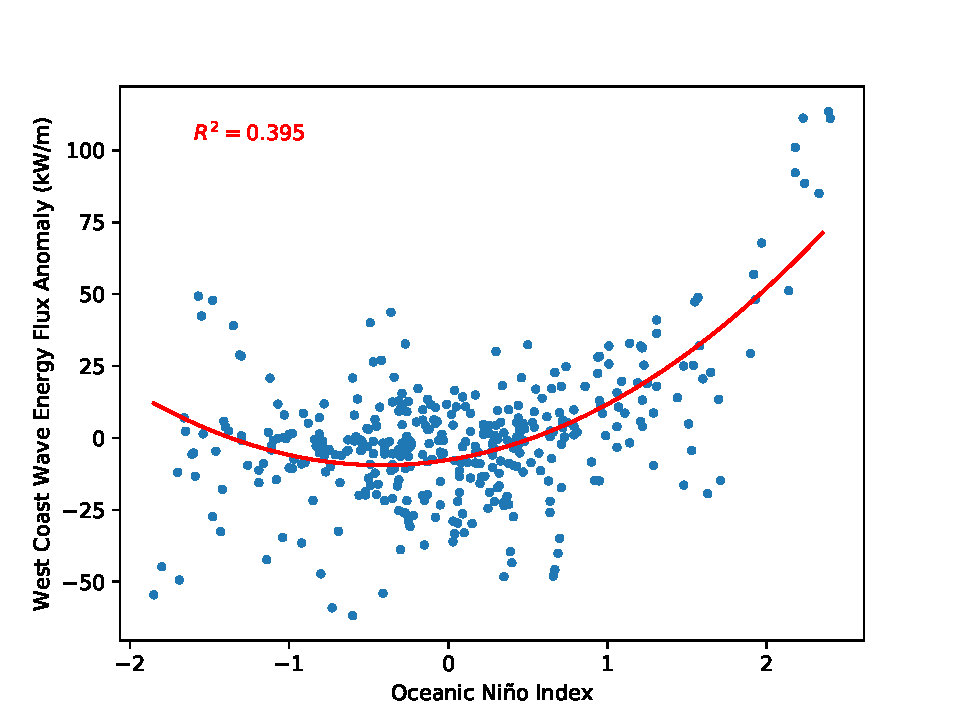
\includegraphics[width=\textwidth]{../fig/ENSO-Comparison.wc.pdf}
  \caption{West Coast wave energy flux anomaly vs. oceanic nino index. The wave energy flux anomaly (annual cycle removed) is averaged along the EEZ boundary, has had a 5-month running average applied, and lags the ONI signal by 2-months.}
  \label{fig:wc-nino}
\end{figure}


\section{Conclusion} \label{sec:conclusion}

We propose a methodology for theoretical wave resource assessment that resolves several outstanding issues with earlier approaches. In particular, this work accounts for wave directionality in order to reduce `double counting', and also includes the energy added to the wave field by local winds. This provides a consistent methodology for accounting for wave energy at national/regional scales. So that policy makers can have a clear understanding of wave energy potential. As other nations/regions adopt the methodology, we will have an apples-to-apples comparison of opportunity, which can inform decision making and investment.

We then apply this methodology to the U.S. EEZ (except for the portion of the EEZ associated with U.S. Pacific Islands Territories), and find that the total U.S. wave energy resource is greater than 3,300 TWh/yr.
\note{We need to decide which `one number' we're going to use here.}
This is an increase of ~25\% compared to earlier DOE wave resource assessments, and is due to the combination of extending the resource area to the edge of the EEZ and incorporating the local resource. The `inner shelf' resource also increases from a total of ~1600 TWh/yr in EPRI 2011 to 1800 TWh/yr here. \note{Most of the increase is in AK. Why?! ... The 'inner shelf' remote resource is > than the EEZ remote resource. Is this just because the contour is longer? Is it worth discussing this nuance in RESULTS or DISCUSSION?}

A detailed assessment of the ``technical resource potential'', which accounts for the efficiency and array design of existing technologies is left for future work. Furthermore, an assessment of the ``practical resource'' is a greater challenge because it requires accounting for regional permitting details, ocean-planning designations, and competing uses by other ocean stakeholders.

We encourage he IEC wave resource assessment team to consider adopting pieces of this methodology in the ``reconaissance'' level assessments in order to promote the use of regional resource assessment that can be compared. Furthermore, the methods proposed here could also be of use to project developers in identifying the maximum resource potential of a project site. \note{Need to think about how to say this more tactfully.}


%%% Local Variables:
%%% TeX-master: "wave_res"
%%% End:
